%%%-------------------------------------------------%%%
%%% Sub document results %%%
%%%-------------------------------------------------%%%

\section{Results}

\textcolor{red}{Gesamtschweizer Grafik (mit imputierten Daten) einmal eine Linie mit Bias, einmal ohne
Kantonsweise Grafiken
Kuznets / U-Turn, Test der Hypothesen mit den final Daten. Der link zwischen rein deskriptiv  und Theorie plus Modell ist aktuell noch ein krasser Drahtseilakt...}

\subsection{Gini coefficients for taxable income, income before deductions and taxable income after tax}

\begin{knitrout}
\definecolor{shadecolor}{rgb}{0.969, 0.969, 0.969}\color{fgcolor}\begin{kframe}
\begin{alltt}
\hlkwd{library}\hlstd{(foreign)}
\hlkwd{library}\hlstd{(ggplot2)}
\hlstd{df} \hlkwb{<-} \hlkwd{read.dta}\hlstd{(}\hlstr{"../../data/ginis_und_perzentile.dta"}\hlstd{)}
\hlstd{df}\hlopt{$}\hlstd{zeros} \hlkwb{<-} \hlstd{df}\hlopt{$}\hlstd{null_norm}\hlopt{/}\hlstd{df}\hlopt{$}\hlstd{cpop}  \hlcom{# i only use normal cases here}
\end{alltt}
\end{kframe}
\end{knitrout}


\begin{knitrout}
\definecolor{shadecolor}{rgb}{0.969, 0.969, 0.969}\color{fgcolor}\begin{kframe}
\begin{alltt}
\hlstd{df}\hlopt{$}\hlstd{G_reink[df}\hlopt{$}\hlstd{G_reink} \hlopt{==} \hlnum{1}\hlstd{]} \hlkwb{<-} \hlnum{NA}
\hlstd{df}\hlopt{$}\hlstd{G_taxed[df}\hlopt{$}\hlstd{G_taxed} \hlopt{==} \hlnum{1}\hlstd{]} \hlkwb{<-} \hlnum{NA}
\hlkwd{library}\hlstd{(reshape)}
\end{alltt}


{\ttfamily\noindent\itshape\color{messagecolor}{\#\# Loading required package: plyr\\\#\# \\\#\# Attaching package: 'reshape'\\\#\# \\\#\# Die folgenden Objekte sind maskiert from 'package:plyr':\\\#\# \\\#\#\ \ \ \  rename, round\_any}}\begin{alltt}
\hlstd{dflong} \hlkwb{<-} \hlkwd{melt}\hlstd{(df[,} \hlkwd{c}\hlstd{(}\hlstr{"G_steink"}\hlstd{,} \hlstr{"G_reink"}\hlstd{,} \hlstr{"G_taxed"}\hlstd{,} \hlstr{"kanton"}\hlstd{,} \hlstr{"steuerperiode"}\hlstd{)],}
    \hlkwc{id} \hlstd{=} \hlkwd{c}\hlstd{(}\hlstr{"kanton"}\hlstd{,} \hlstr{"steuerperiode"}\hlstd{))}
\hlkwd{names}\hlstd{(dflong)[}\hlnum{3}\hlstd{]} \hlkwb{<-} \hlstr{"Type"}
\hlkwd{names}\hlstd{(dflong)[}\hlnum{4}\hlstd{]} \hlkwb{<-} \hlstr{"Gini"}
\hlkwd{levels}\hlstd{(dflong}\hlopt{$}\hlstd{Type)} \hlkwb{<-} \hlkwd{c}\hlstd{(}\hlstr{"taxable income"}\hlstd{,} \hlstr{"income before deductions"}\hlstd{,} \hlstr{"taxable income after tax"}\hlstd{)}
\hlkwd{ggplot}\hlstd{(dflong[dflong}\hlopt{$}\hlstd{kanton} \hlopt{==} \hlstr{"CH"}\hlstd{, ],} \hlkwd{aes}\hlstd{(}\hlkwc{x} \hlstd{= steuerperiode,} \hlkwc{y} \hlstd{= Gini,} \hlkwc{colour} \hlstd{= Type))} \hlopt{+}
    \hlkwd{geom_line}\hlstd{(}\hlkwc{size} \hlstd{=} \hlnum{1}\hlstd{)} \hlopt{+} \hlkwd{theme_bw}\hlstd{()} \hlopt{+} \hlkwd{xlab}\hlstd{(}\hlstr{"tax period"}\hlstd{)}
\end{alltt}
\end{kframe}
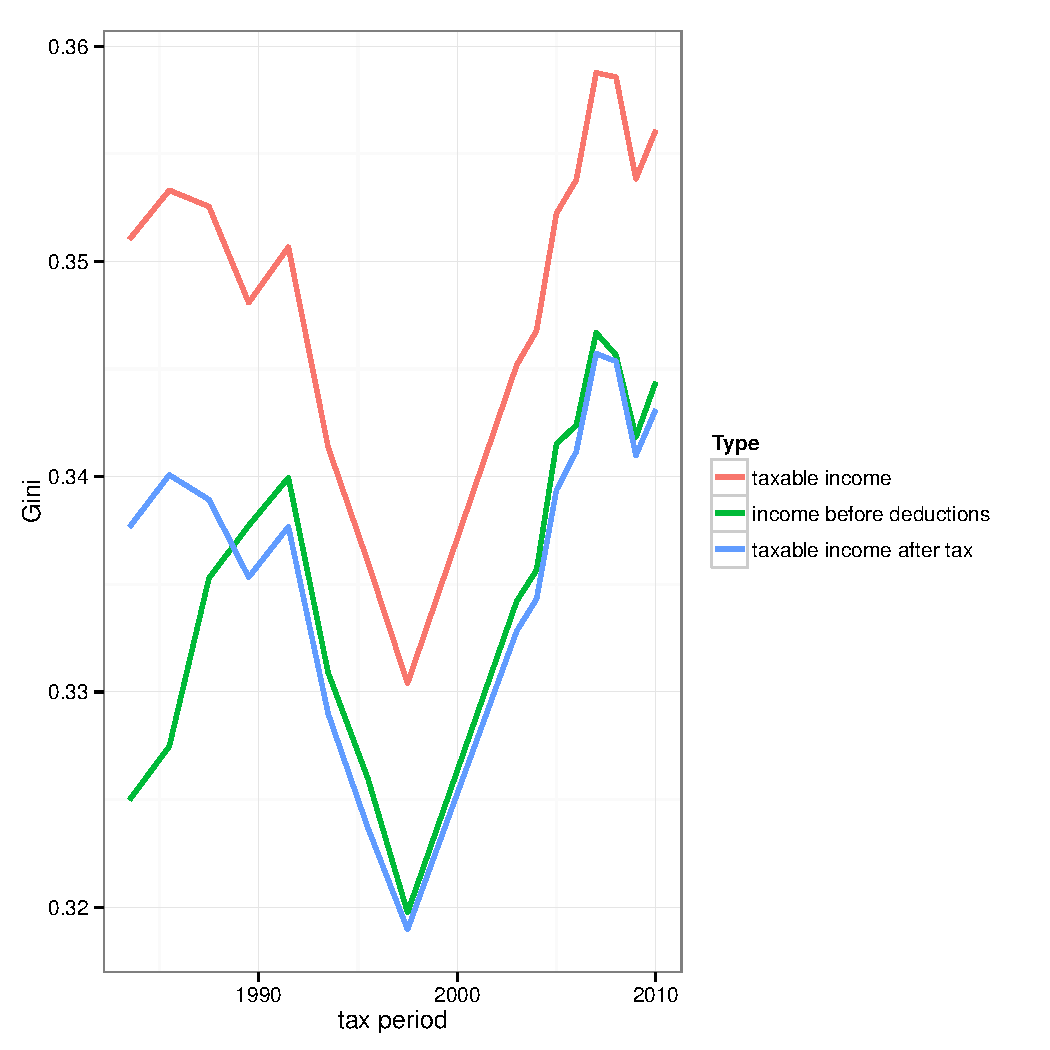
\includegraphics[width=\maxwidth]{figure/different_ginis1} 
\begin{kframe}\begin{alltt}
\hlkwd{ggplot}\hlstd{(dflong,} \hlkwd{aes}\hlstd{(}\hlkwc{x} \hlstd{= steuerperiode,} \hlkwc{y} \hlstd{= Gini,} \hlkwc{colour} \hlstd{= Type))} \hlopt{+} \hlkwd{geom_line}\hlstd{()} \hlopt{+}
    \hlkwd{facet_wrap}\hlstd{(}\hlopt{~}\hlstd{kanton)} \hlopt{+} \hlkwd{theme_bw}\hlstd{()} \hlopt{+} \hlkwd{xlab}\hlstd{(}\hlstr{"tax period"}\hlstd{)}
\end{alltt}
\end{kframe}
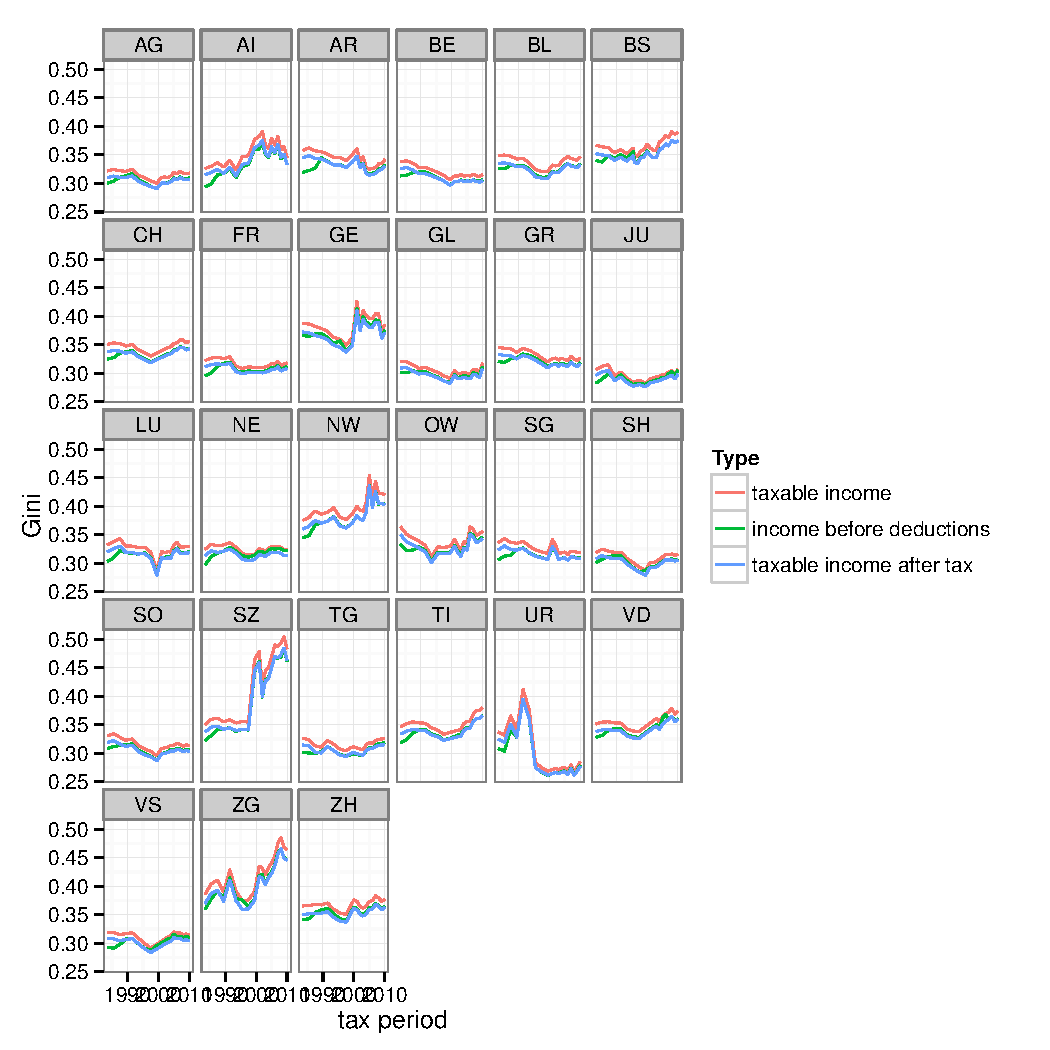
\includegraphics[width=\maxwidth]{figure/different_ginis2} 

\end{knitrout}


\subsection{Zero share}

Estimation using population statistics (1945/46-1993/94) and official tax administration statistics (1995/96 and later) 


\subsection{Income measures with and without zeros}

taxable income with and without zeros

\begin{knitrout}
\definecolor{shadecolor}{rgb}{0.969, 0.969, 0.969}\color{fgcolor}\begin{kframe}
\begin{alltt}
\hlstd{dflong} \hlkwb{<-} \hlkwd{melt}\hlstd{(df[,} \hlkwd{c}\hlstd{(}\hlstr{"G_steink"}\hlstd{,} \hlstr{"G_steink0"}\hlstd{,} \hlstr{"kanton"}\hlstd{,} \hlstr{"steuerperiode"}\hlstd{)],}
    \hlkwc{id} \hlstd{=} \hlkwd{c}\hlstd{(}\hlstr{"kanton"}\hlstd{,} \hlstr{"steuerperiode"}\hlstd{))}
\hlkwd{names}\hlstd{(dflong)[}\hlnum{3}\hlstd{]} \hlkwb{<-} \hlstr{"Type"}
\hlkwd{names}\hlstd{(dflong)[}\hlnum{4}\hlstd{]} \hlkwb{<-} \hlstr{"Gini"}
\hlkwd{levels}\hlstd{(dflong}\hlopt{$}\hlstd{Type)} \hlkwb{<-} \hlkwd{c}\hlstd{(}\hlstr{"without zeros"}\hlstd{,} \hlstr{"including zeros"}\hlstd{)}
\hlkwd{ggplot}\hlstd{(dflong[dflong}\hlopt{$}\hlstd{kanton} \hlopt{==} \hlstr{"CH"} \hlopt{&} \hlstd{dflong}\hlopt{$}\hlstd{steuerperiode} \hlopt{>=} \hlnum{1995.5}\hlstd{, ],} \hlkwd{aes}\hlstd{(}\hlkwc{x} \hlstd{= steuerperiode,}
    \hlkwc{y} \hlstd{= Gini,} \hlkwc{colour} \hlstd{= Type))} \hlopt{+} \hlkwd{geom_line}\hlstd{(}\hlkwc{size} \hlstd{=} \hlnum{1}\hlstd{)} \hlopt{+} \hlkwd{theme_bw}\hlstd{()} \hlopt{+} \hlkwd{xlab}\hlstd{(}\hlstr{"tax period"}\hlstd{)}
\end{alltt}
\end{kframe}
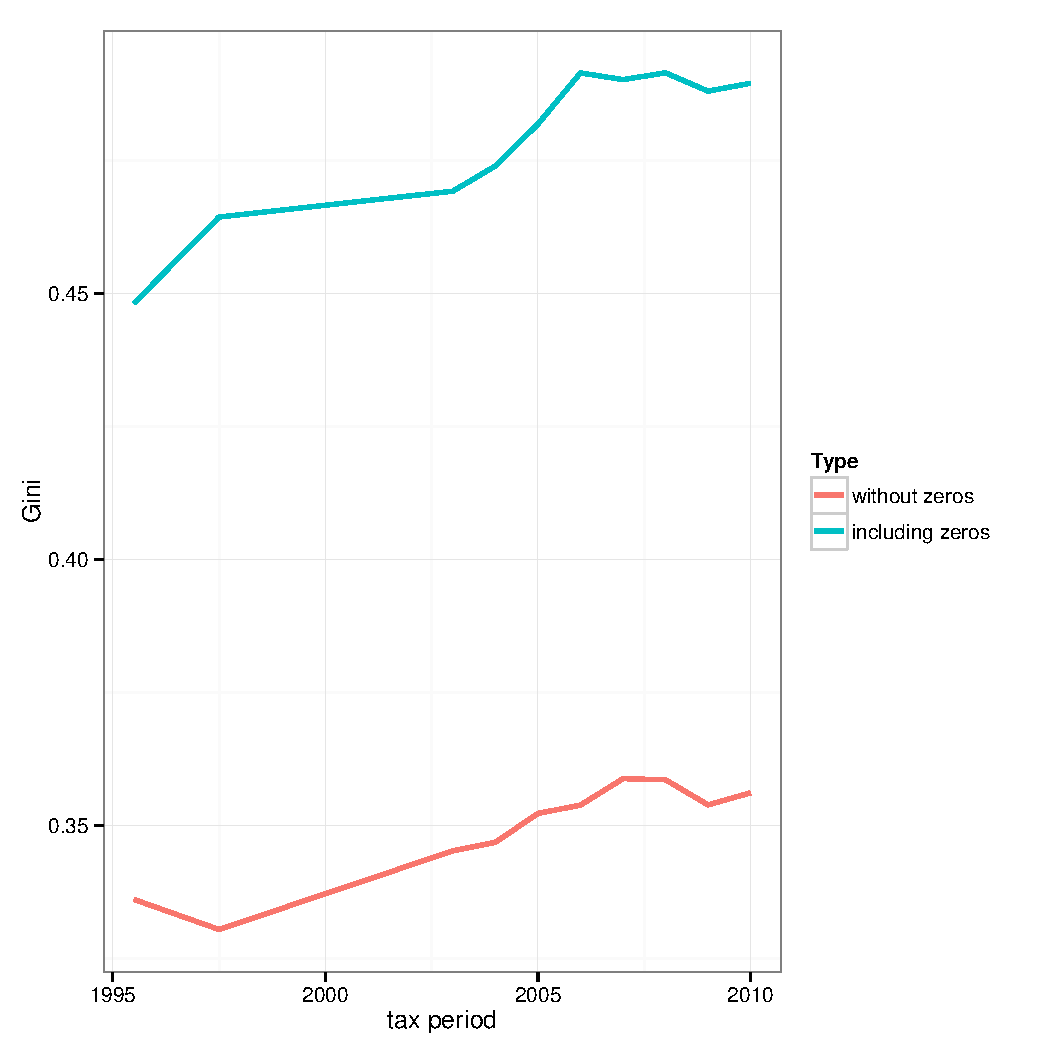
\includegraphics[width=\maxwidth]{figure/with_without_zeros1} 
\begin{kframe}\begin{alltt}
\hlkwd{ggplot}\hlstd{(dflong[dflong}\hlopt{$}\hlstd{steuerperiode} \hlopt{>=} \hlnum{1995.5}\hlstd{, ],} \hlkwd{aes}\hlstd{(}\hlkwc{x} \hlstd{= steuerperiode,} \hlkwc{y} \hlstd{= Gini,}
    \hlkwc{colour} \hlstd{= Type))} \hlopt{+} \hlkwd{geom_line}\hlstd{()} \hlopt{+} \hlkwd{facet_wrap}\hlstd{(}\hlopt{~}\hlstd{kanton)} \hlopt{+} \hlkwd{theme_bw}\hlstd{()} \hlopt{+} \hlkwd{xlab}\hlstd{(}\hlstr{"tax period"}\hlstd{)} \hlopt{+}
    \hlkwd{opts}\hlstd{(}\hlkwc{axis.text.x} \hlstd{=} \hlkwd{theme_text}\hlstd{(}\hlkwc{angle} \hlstd{=} \hlnum{60}\hlstd{))}
\end{alltt}


{\ttfamily\noindent\itshape\color{messagecolor}{\#\# 'opts' is deprecated. Use 'theme' instead. (Deprecated; last used in version 0.9.1)\\\#\# theme\_text is deprecated. Use 'element\_text' instead. (Deprecated; last used in version 0.9.1)}}\end{kframe}
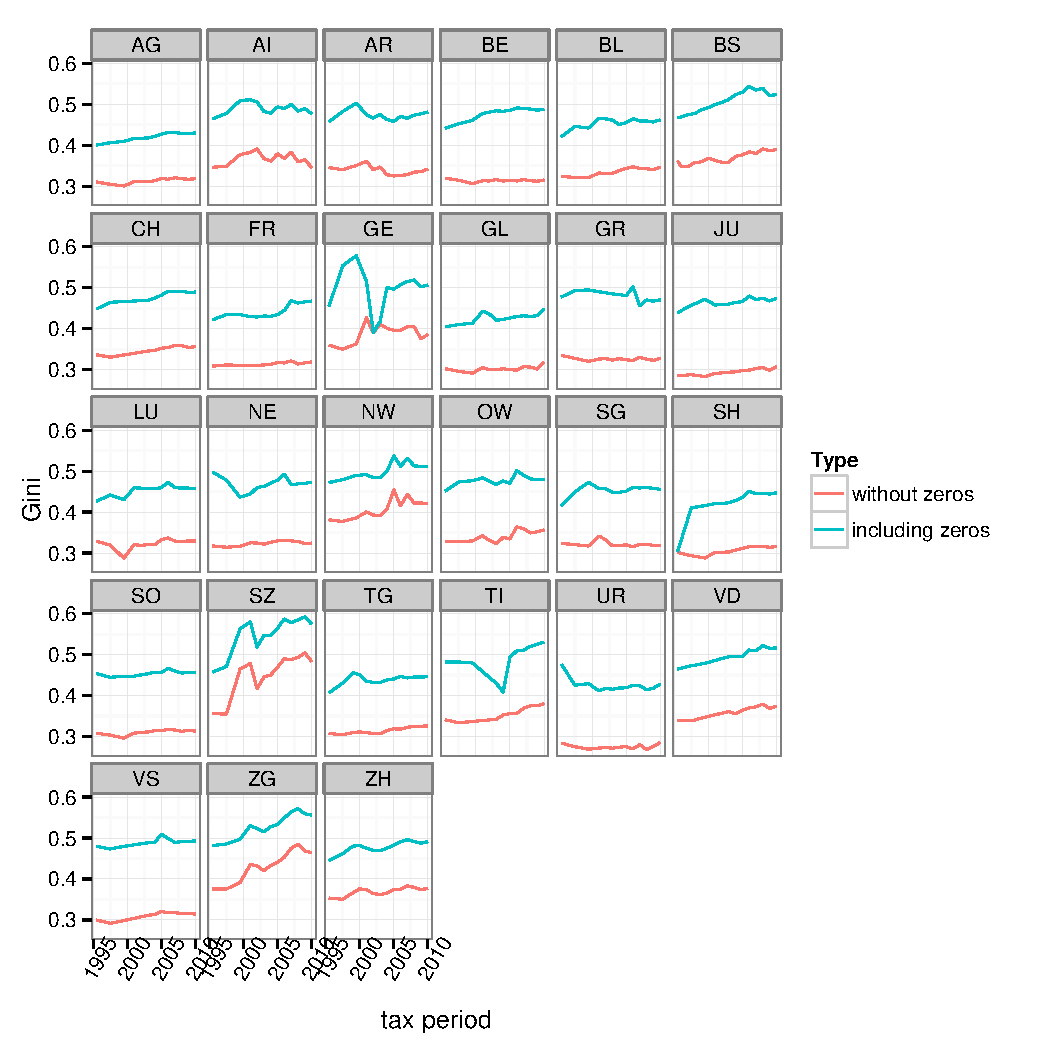
\includegraphics[width=\maxwidth]{figure/with_without_zeros2} 

\end{knitrout}


Including zeros leads to significantly higher gini coefficients. However we must keep in mind, that these might be artifically high values as we assume zero income for everyone in the zero group. We can conclude more from the graphic: the ratio between both measures seems to be quite constant although for aggregate Switzerland but there are minor deviations for multiple cantons as well as strong deviations for the cantons Geneva and Tessin. However the problems seem not to result from a shift in the zero-share over time but they are specific for the time-period when the tax system changed. 

%Switzerland (income and wealth)
%- graph with gini over time> identify periods of change
%- closer look at interesting periods with relative distribution methods-> is change because of down- or upgrading?
%Cantonal level (income and wealth)
%- different development on regional level 
%Switzerland in international comparison
%- Comparison with other data sources- LIS (inequality in Switzerland is decreasing, which is quite special, because the common pattern in western countries shows an increase in inequality

%- Comparison with other countries (similar data)


% Es scheinen mir aktuell etwas viele Ergebnisse zu sein und ich frage mich, ob wir Ergebnisse auf der Kantonsebene ausklammern sollen. Wenn wir drei Ergebniss haben (1) Unterscheidung von unterschiedlichen Perioden der Ungleichheitsentwicklung (2) Beurteilung dieser Perioden hinsichtlich dem Bereich der Veränderungen (Arme, Reiceh) und Entwicklung der Vermögensungleichheit, dann haben wir bereits viel. Falls wir spezifische Erkenntnisse nur aus dem Kantonsvergleich bekommen (Bias durch Nuller o.ä.), dann sollten wir trotzdem damit arbeiten.

%rf: genau. kantone unterstreichen die probleme mit dem 0er bias und die probleme mit "imputing the gap". mehr muss erstmal nicht sein.


